\chapter{Nearest Neighbors}
\section{Introduction}
Unlike the Bayes' rule, the family of algorithms called $k$-NN ( $k$ Nearest Neighbors) does not use the probability theory. It also ranks among time-tested methods, successful (as well as sometimes regrettably unsuccessful) in many applications.

The $k$-NN algorithm is based on using similarity - the principal idea is that similar items belong to the same class. Therefore, it is necessary just to collect and store the convenient number of labeled samples belonging to each relevant class - and the training phase is completed. This is undoubtedly a big advantage of the $k$-NN algorithm: very fast and simple training procedure. In addition, it is a reason why $k$-NN is counted among the so-called \textit{lazy algorithms}. A good discussion about $k$-NN can be found in \cite{ref76}.

During the classification process, $k$-NN waits for an incoming unlabeled item, finds its $k \geq 1$ most similar labeled sample(s) and assigns the appropriate label to the unlabeled item. Unlike the training phase, the classification one is typically much more demanding and often computationally complex due to the time-consuming similarity determination of a classified item in relation to every stored sample. More samples naturally means more information; however, also more computation including its non-linearly increasing complexity, which depends on the sample number as well as on the dimensionality extent.

\section{Similarity as Distance}
If an unlabeled item $x_{i}$ is the most similar (or identical) to a certain labeled sample $s_{j}$, then $x_{i}$ is labeled just as $s_{j}: s_{j} \in C_{l}, x_{i} \sim s_{j} \rightarrow x_{i} \in C_{l}$, or in other words, $C_{l} \subset C_{l} \cap x_{i}$, where $C_{l}$ is one of classes appropriate to the analyzed problem. Thus. the element $s_{j}$ is called the nearest neighbor of $x_{i}$.

This is, basically a very simple algorithm; however, the question is, how to compute that similarity.? Several methods of the numeric expression of similarity, which are based on computing a kind of distance between pairs of points, which represent individual samples in an $n$-dimensional space may be used. Depending on the properties of the space under consideration, there are numerous methods for calculating the distance.

Euclidean distance: The commonly known and habitually used distance named after the 'founder of geometry,' the ancient Greek mathematician Eukleides (Euclid) of Alexandria (born c. 325 BC, died c. 270 BC). This distance is the straight-line distance between two points in Euclidean space, which is the two-dimensional plane and three-dimensional space, i.e., it can be the $n$-dimensional hyperplane using the Cartesian coordinate system. To compute the Euclidean distance $d_{E}$ between a point $A$ with $n$ coordinates $a_{1}, a_{2}, \ldots, a_{n}$, and a point $B$ with coordinates $b_{1}, b_{2}, \ldots, b_{n}$, the familiar formula is applied:

\begin{equation*}
d_{E}(A, B)=\sqrt{\left(a_{1}-b_{1}\right)^{2}+\left(a_{2}-b_{2}\right)^{2}+\ldots+\left(a_{n}-b_{n}\right)^{2}}=\sqrt{\sum_{i=1}^{n}\left(a_{i}-b_{i}\right)^{2}} \tag{6.1}
\end{equation*}


Manhattan distance: The distance between two points is the sum of the absolute differences of their Cartesian coordinates. This distance $d_{M}$, named after the layout of most streets on the island of Manhattan (a borough of New York City), is an alternative to the Euclidean distance when it is possible to move in the space only in parallel with mutually perpendicular axes:


\begin{equation*}
d_{M}(A, B)=\left|a_{1}-b_{1}\right|+\left|a_{2}-b_{2}\right|+\ldots+\left|a_{n}-b_{n}\right|=\sum_{i=1}^{n}\left|a_{i}-b_{i}\right| \tag{6.2}
\end{equation*}

Hamming distance: A very simple distance between two strings (or vectors) of equal length, which is the number of positions at which the corresponding symbols are either equal or different. The more different the symbols, the less similar (or more distant) the strings. The Hamming distance, named after a mathematician Richard Wesley Hamming ( $11^{\text {th }}$ February 1915-7 ${ }^{\text {th }}$ January 1998), can also be used to determine the similarity or difference between two text documents when the representation of words is binary (for example, using symbols 1 and 0 , for when a word occurs $=1$, and a word does not occur $=0$ ) provided that all such represented documents employ the same joint vocabulary (which guarantees the required same length of vector).

\textit{Mahalanobis distance}: Named after an Indian statistician, Prasanta Chandra Mahalanobis ( $29^{\text {th }}$ June 1893-28 ${ }^{\text {th }}$ June 1972), the distance used in statistics. It measures a point distance from a mean of a distribution using covariance matrix. It might be useful when there is correlation between points representing training documents.

Cosine distance: This similarity can be used in text mining when documents with very different number of words are compared, in which case the scalar frequency representation (coordinates of a point) may not provide reliable results; for example, an abstract of an article and the article itself, or a short review compared to a long one expressing the same opinion. In such a case, each document is taken as a non-zero vector pointing from the origin of the coordinate system to its endpoint given by the coordinates and the mutual similarity is measured by the angle between pairs of the vectors. If the angle $\alpha$ between two vectors is zero, they are considered to be identical because $\cos \left(0^{\circ}\right)=1.0$ (or $100 \%$ similarity). If $\alpha=90^{\circ}$, then $\cos \left(90^{\circ}\right)=0.0$ (or complete dissimilarity). Otherwise, for $0^{\circ}<\alpha<90^{\circ}$, the similarity is something in between. Note that any distance or frequency cannot be negative, therefore no negative cosine values are used.

The cosine similarity for two vectors $\mathbf{x}_{j}$ and $\mathbf{x}_{k}$ can be written as the following formula:


\begin{equation*}
\cos (\alpha)=\frac{\mathbf{x}_{j} \cdot \mathbf{x}_{k}}{\left\|\mathbf{x}_{j}\right\|\left\|\mathbf{x}_{k}\right\|}=\frac{\sum_{i=1}^{n} x_{j_{i}} \cdot x_{k i}}{\sqrt{\sum_{i=1}^{n} x_{j i}^{2}} \sqrt{\sum_{i=1}^{n} x_{k_{i}}^{2}}} \tag{6.3}
\end{equation*}

Figure 6.1 illustrates a very simple case. There are three documents doc ${ }_{1}$, $\mathrm{doc}_{2}$, and $\mathrm{doc}_{3}$. The vocabulary space is limited to just two words $w_{i}$ and $w_{j}$ represented by their frequencies in the documents, $f_{w_{i}}$ and $f_{w_{j}}$, respectively. The documents $\operatorname{doc}_{1}$ and $\operatorname{doc}_{2}$ have different absolute numbers of the two word

\begin{figure}[!ht]
\begin{center}
  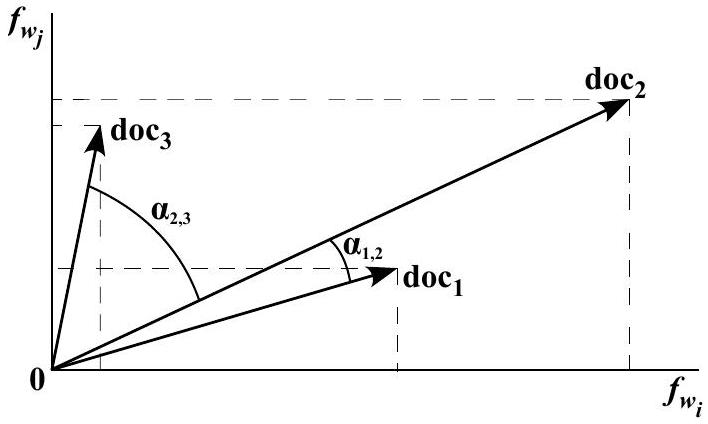
\includegraphics[width = 0.55\textwidth]{chapter/chapter6/2025_10_21_5ba6420d88ee7388cb5eg-180.jpg}
\caption{The illustration of the cosine distance (similarity) between documents represented by vectors. A simplified two-dimensional space with frequencies of $word_{i}$ and $word_{j}$.frequencies, however, their rate $f_{w_{i}}: f_{w_{j}}$ is almost the same for both documents. From the Euclidean point of view, the documents are far apart, hence different.}

\end{center}
\end{figure}

On the contrary, from the cosine similarity point of view, they are very close, because the $\alpha_{1,2}$ angle between them is considerably small. The document doc ${ }_{3}$ contains only a small number of words $w_{i}$ and, in addition, the $\operatorname{doc}_{3}$ frequency rate $f_{w_{i}}: f_{w_{j}}$ differs from both $\operatorname{doc}_{1}$ and $\operatorname{doc}_{2}$ rates which is also the reason for the big angle $\alpha_{2,3}$ and significant dissimilarity apart from the Euclidean viewpoint.

An interested reader can find much deeper description of various distance/similarity methods including their details in, for example, \cite{ref156} and \cite{ref212}.

\section{Illustrative Example of \texorpdfstring{$\boldsymbol{k}$}{k}-NN}
The small and simple data set, which consists of seven textual documents related to the weather description (introduced earlier in the section 5.5 Illustrative Example of Naïve Bayes) can illustrate the application of the $k$-NN algorithm to classification. The frequencies of the seven vocabulary words in the individual documents act as coordinates of the documents in a seven-dimensional abstract space (seven attributes/variables $w_{1}=\mathrm{it}, w_{2}=\mathrm{is}, \ldots, w_{7}=$ very). Each of the seven training documents is represented as a point in that space labeled by its class name, either pos or neg.

The classified document position in the space is known, too, thus it is necessary to find the nearest point, which is labeled, and to then assign that label to the unlabeled item.

The training data-set with an added sequence number, No.:

\begin{flushleft}
\begin{tabular}{rrrrrrrrr}
No. & it, & is, & nice, & weather, & cold, & not, & very, & class \\
1. & 1, & 1, & 1, & 1, & 0, & 0, & 0, & pos\\
2. & 1, & 1, & 0, & 0, & 1, & 0, & 0, & neg\\
3. & 1, & 1, & 0, & 0, & 1, & 1, & 1, & pos\\
4. & 0, & 0, & 1, & 0, & 0, & 1, & 0, & neg\\
5. & 0, & 0, & 0, & 0, & 1, & 0, & 1, & neg\\
6. & 0, & 0, & 0, & 0, & 1, & 0, & 0, & neg\\
7. & 0, & 0, & 1, & 1, & 0, & 0, & 1, & pos\\
\end{tabular}
\end{flushleft}

The unlabeled document calling for its classification (the mark '?' stands here for an unknown label) looks like this:

$$
1, \quad 1, \quad 1, \quad 0, \quad 1, \quad 1, \quad 0, \quad \text { ? }
$$

Provided that there is no reason to avoid the Euclidean space, the distances of the classified point from the labeled samples can be computed and then the nearest sample's label may be used. Due to the simplicity of the training dataset, the frequencies here are only 0 's or 1 's, but that does not change anything.

For the first training document, its Euclidean distance $d_{1}$ from the classified point is:

$$
\begin{gathered}
\sqrt{(1-1)^{2}+(1-1)^{2}+(1-1)^{2}+(0-1)^{2}+(1-0)^{2}+(1-0)^{2}+(0-0)^{2}}= \\
=\sqrt{3} \doteq 1.73 .
\end{gathered}
$$

Similarly, all the six remaining distances (from the $2^{\text {nd }}$ up to the $7^{\text {th }}$ training sample) are calculated as well: $d_{2}=1.41, d_{3}=1.41, d_{4}=1.73, d_{5}=2.24, d_{6}=$ 2.0 , and $d_{7}=2.45$.

Evidently, the shortest distance is 1.41 - unfortunately, it is shared by two training neighbors (the $2^{\text {nd }}$ and $3^{\text {rd }}$ ), each one from a different class.

So, 1-NN does not work (nor 2-NN), it is an irresolute case. What about 3-NN? This is again a draw, there are two candidates for it (the $1^{\text {st }}$ and $4^{\text {th }}$ ) having the same distance 1.73. We could consider 5-NN. Adding the sample No. 6 with its distance 2.0 and label neg, there are now two positive and three negative samples; therefore, the voting majority finally decides: the classified item gets the label, \textit{neg}.

As there are only word frequencies like 0 and 1 , it is possible to employ the computationally simpler binary representation together with the Hamming distance.

Evidently, the distances, $d$, between the unlabeled example and the samples No. 1 to 7 , are $3,2,2,3,5,4$, and 6 , respectively. The closest samples are No. 2 ( $d=2$. neg) and No. $3(d=2, p o s)$ so the result is a draw. After adding the next closest neighbors No. 1 (pos) and No. 4 (neg) with $d=3$, that is, a draw again. The closest neighbor which follows is No. 6 (neg) with $d=4$, thus the rate is 3 neg : 2 pos, so the assigned label is neg.

This illustration shows a possible disadvantage of $k$-NN, namely the difficulty in determining the number $k$ of neighbors in advance. In practice, a researcher often has to determine the right number of nearest neighbors experimentally.

In any case, at the beginning, all the distances between the unlabeled point and the points with labels must be calculated, they must then be ordered by size, and finally, used for the decision.

If the close neighbourhood for small $k$ 's gives poor results, the surroundings of an unlabeled point should be enlarged (increasing $k$ ). It is, however, necessary to be cautious if just a narrow majority prevails because, for example, a result 50:51 (for $k=101$ ) is less compelling than $2: 1(k=3)$ or $3: 2$ or $4: 1(k=5)$, even if it may be correct and acceptable - it depends on a particular application and its data type. When in doubt, the results of alternative algorithms might be taken in account, even if only for comparison.

The correct nearest neighbor selection may be affected by grossly different scale ratios on the axes. If justified reasons do not preclude it, it is advisable to normalize the scales on the axes to, for example, the interval $[0,1]$ :

$$
\xi_{i}=\frac{x_{i}-\min \left(x_{i}\right)}{\max \left(x_{i}\right)-\min \left(x_{i}\right)},
$$

where $\xi_{i}$ is a normalized value of $x_{i}, \min \left(x_{i}\right)$ is the minimum value and $\max \left(x_{i}\right)$ the maximum value on a given axis obtained from the training samples. The illustration, Figure 6.2, shows how a classified case (marked with '?') can change its classification from a class B to a class A due to normalization of scales. The need for normalization can, in case of doubt, be confirmed or rejected by the testing procedure.

It is also worth mentioning here other possible problems concerning (not only) $k$-NN, namely the influence of a very high-dimensional space on classification results, where, for example, the influence of a relevant attribute can be overridden by a large number of irrelevant ones, as seen in \cite{ref96}.

\begin{figure}[!ht]
\begin{center}
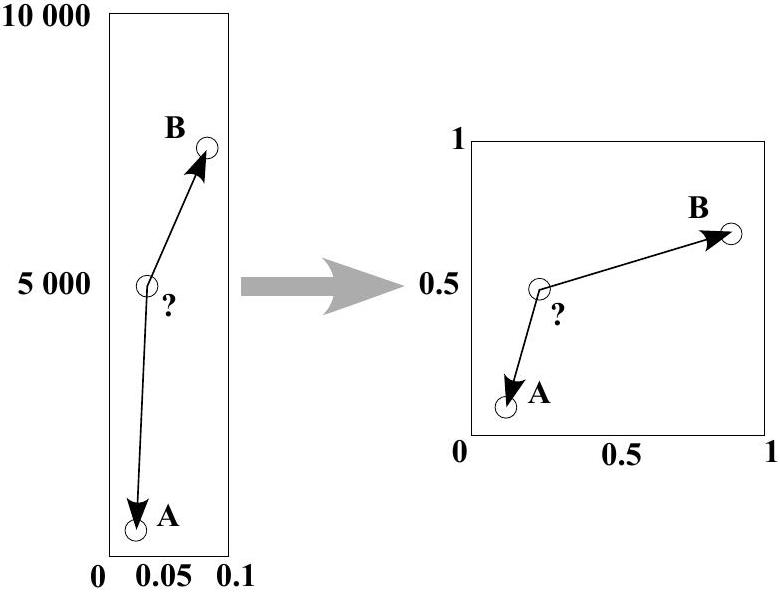
\includegraphics[width=0.6\textwidth]{chapter/chapter6/2025_10_21_5ba6420d88ee7388cb5eg-183.jpg}
\caption{Very different scale ratios (on the left side) of different dimensions may cause the nearest neighbor to be incorrectly identified. After normalization (on the right side), the situation may be quite the opposite.}
\end{center}
\end{figure}

\section{\textit{k}-NN in R}
The two examples which follow demonstrate the simple application of the $k$-NN algorithm to the same data, BookReviews.csv, as in the previous chapters. The R classification library called class and just one neighbor ( $k=1$ ) are used. Alter-\\
natively, the reader may simply try to change the parameter $k$ to see if a higher number of neighbors will provide better classification results (accuracy). The first sample uses a test set:

\begin{verbatim}
library(class)
# loading the data
data <- read.csv('BookReviews.csv', header=TRUE)

# converting the data to a matrix
dtm <- as.matrix(data)

# removing the object data (unnecessary from now)
rm(data)

# number of instances
n <- dim(dtm)[1]

# number of attributes
m <- dim(dtm)[2]

# indexes of 100 testing samples
number_of_test_samples <- 100
test_index <- 1:number_of_test_samples

# selecting training samples
train_data <- dtm[-test_index, 1:(m-1)]
train_labels <- dtm[-test_index, m]

# selecting testing samples
test_data <- dtm[test_index, 1:(m-1)]
test_labels <- dtm[test_index, m]

# training a k-nearest neighbors model
knn_model <- knn(train_data, test_data, train_labels, k=1)

# creating a confusion matrix
cm <- table(test_labels, knn_model)
print("Confusion matrix")
print(cm)
\end{verbatim}

\begin{verbatim}
# number of instances
n <- sum(cm)

# number of correctly classified instances for each class
correct <- diag(cm)

# numbers of instances in each class
instances_in_classes <- apply(cm, 1, sum)

# numbers of each class predictions
class_predictions <- apply(cm, 2, sum)

# accuracy
accuracy <- sum(correct)/n

# precision per class
precision <- correct/class_predictions

# recall per class
recall <- correct/instances_in_classes

# F1-measure per class
f1 <- 2 * precision * recall / (precision + recall)

# printing summary information for all classes
df <- data.frame(precision, recall, f1)
print("Detailed classification metrics")
print(df)
print(paste("Accuracy:", accuracy))

# macroaveraging
print("Macro-averaged metrics")
print(colMeans(df))

# microaveraging
print("Micro-averaged metrics")
print(apply(df, 2, function (x)
    weighted.mean(x, w=instances_in_classes)))
\end{verbatim}

The console output after a successful run:

\hspace{-0.3cm}[1] "Confusion matrix" \\

\hspace{2cm}knn\_mode

\begin{flushleft}
\begin{tabular}{lll}
test\_labels & 0 & 1 \\
0 & 35 & 22 \\
1 & 15 & 28 \\
\end{tabular}
\end{flushleft}

\begin{flushleft}
\begin{tabular}{rrrr}
\multicolumn{4}{l}{[1] "Detailed classification metrics"} \\
 & precision & recall & f1 \\
0 & 0.70 & 0.6140351 & 0.6542056 \\
1 & 0.56 & 0.6511628 & 0.6021505 \\
\end{tabular}
\end{flushleft}
\hspace{0.3cm}[1] "Accuracy: 0.63"\\[0pt]

\hspace{-0.3cm}[1] "Macro-averaged metrics"

\begin{flushleft}
\begin{tabular}{rrr}
precision & recall & f1 \\
0.6300000 & 0.6325989 & 0.6281781 \\
\end{tabular}
\end{flushleft}

\hspace{-0.3cm}[1] "Micro-averaged metrics"

\begin{flushleft}
\begin{tabular}{rrr}
precision & recall & f1 \\
0.6398000 & 0.6300000 & 0.6318219 \\
\end{tabular}
\end{flushleft}

The output from $k$-NN classification using the cross-validation testing follows:

\begin{verbatim}
Cross-validation fold: 1
    Accuracy: 0.64
    Precision(positive): 0.5714286
    Precision(negative): 0.7058824
Cross-validation fold: 2
    Accuracy: 0.59
    Precision(positive): 0.6222222
    Precision(negative): 0.5636364
Cross-validation fold: 3
    Accuracy: 0.56
    Precision(positive): 0.5957447
    Precision(negative): 0.5283019
    Cross-validation fold: 4
    Accuracy: 0.55
    Precision(positive): 0.5102041
    Precision(negative): 0.5882353
\end{verbatim}

\begin{verbatim}
Cross-validation fold: 5
    Accuracy: 0.56
    Precision(positive): 0.5686275
    Precision(negative): 0.5510204
Cross-validation fold: 6
    Accuracy: 0.58
    Precision(positive): 0.5901639
    Precision(negative): 0.5641026
Cross-validation fold: 7
    Accuracy: 0.58
    Precision(positive): 0.4878049
    Precision(negative): 0.6440678
Cross-validation fold: 8
    Accuracy: 0.62
    Precision(positive): 0.6470588
    Precision(negative): 0.5918367
Cross-validation fold: 9
    Accuracy: 0.5
    Precision(positive): 0.5111111
    Precision(negative): 0.4909091
Cross-validation fold: 10
    Accuracy: 0.51
    Precision(positive): 0.6052632
    Precision(negative): 0.4516129
Average Accuracy: 56.9 %
SEM: 1.38
\end{verbatim}

The reader can see the rather different results between the two different training and testing methods demonstrated above. This can be expected because the training and testing examples are not the same, indicating, among other things, that the selected classifier is not robust enough for the data. In such cases, a deeper analysis can be recommended to find answers to questions as to whether the training data is sufficiently representative, if the amount of data is sufficient, or if the selected classification algorithm is appropriate for the given task and should not it be replaced by a more suitable one.